\section{Date: 2026-10-28}
\noindent \textbf{Series ID: DTCORVHFNM} 

\noindent This series is titled Consumer Motor Vehicle Leases Owned by Finance Companies, Level and has a frequency of Monthly. The units are Millions of Dollars and the seasonal adjustment is Not Seasonally Adjusted.The observation start date is 1980-06-01 and the observation end date is 2026-07-01.The popularity of this series is 13. \\ 

\noindent \textbf{Series ID: OMBFRIM027SBOG} 

\noindent This series is titled Other Securities: Mortgage-Backed Securities, Foreign-Related Institutions and has a frequency of Monthly. The units are Billions of U.S. Dollars and the seasonal adjustment is Seasonally Adjusted.The observation start date is 2009-07-01 and the observation end date is 2026-09-01.The popularity of this series is 1. \\ 

\subsection{Raw Regression}
\noindent Regresses the two series against each other directly. A significant result here can come just as easily from both series sharing a long-run trend as from any real relationship.

\begin{center}
\begin{tabular}{lclc}
\toprule
\textbf{Dep. Variable:}          & value\_fred\_OMBFRIM027SBOG & \textbf{  R-squared:         } &     0.811   \\
\textbf{Model:}                  &             OLS             & \textbf{  Adj. R-squared:    } &     0.810   \\
\textbf{Method:}                 &        Least Squares        & \textbf{  F-statistic:       } &     872.2   \\
\textbf{Date:}                   &       Wed, 28 Oct 2026      & \textbf{  Prob (F-statistic):} &  2.03e-75   \\
\textbf{Time:}                   &           17:29:33          & \textbf{  Log-Likelihood:    } &   -373.28   \\
\textbf{No. Observations:}       &               205           & \textbf{  AIC:               } &     750.6   \\
\textbf{Df Residuals:}           &               203           & \textbf{  BIC:               } &     757.2   \\
\textbf{Df Model:}               &                 1           & \textbf{                     } &             \\
\textbf{Covariance Type:}        &          nonrobust          & \textbf{                     } &             \\
\bottomrule
\end{tabular}
\begin{tabular}{lcccccc}
                                 & \textbf{coef} & \textbf{std err} & \textbf{t} & \textbf{P$> |$t$|$} & \textbf{[0.025} & \textbf{0.975]}  \\
\midrule
\textbf{const}                   &      17.1997  &        0.459     &    37.497  &         0.000        &       16.295    &       18.104     \\
\textbf{value\_fred\_DTCORVHFNM} &   -7.456e-05  &     2.52e-06     &   -29.533  &         0.000        &    -7.95e-05    &    -6.96e-05     \\
\bottomrule
\end{tabular}
\begin{tabular}{lclc}
\textbf{Omnibus:}       & 20.349 & \textbf{  Durbin-Watson:     } &    0.152  \\
\textbf{Prob(Omnibus):} &  0.000 & \textbf{  Jarque-Bera (JB):  } &   23.791  \\
\textbf{Skew:}          &  0.816 & \textbf{  Prob(JB):          } & 6.82e-06  \\
\textbf{Kurtosis:}      &  2.650 & \textbf{  Cond. No.          } & 7.94e+05  \\
\bottomrule
\end{tabular}
%\caption{OLS Regression Results}
\end{center}

Notes: \newline
 [1] Standard Errors assume that the covariance matrix of the errors is correctly specified. \newline
 [2] The condition number is large, 7.94e+05. This might indicate that there are \newline
 strong multicollinearity or other numerical problems.

\begin{figure}
\centering
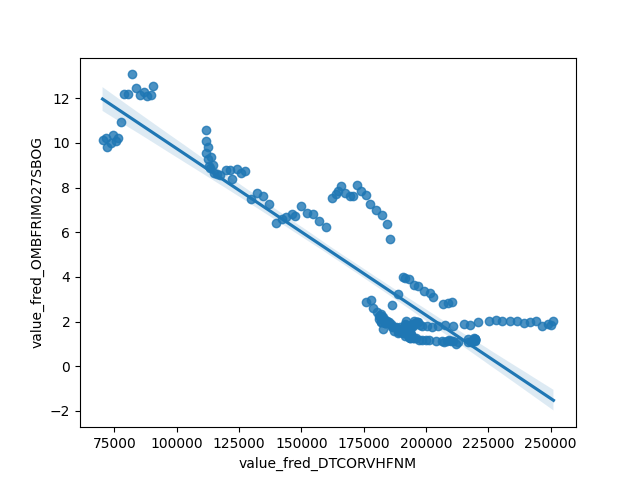
\includegraphics[scale = 0.9]{plots/plot_2026-10-28.png}
\caption{Raw Regression Plot for 2026-10-28}
\end{figure}
\newpage
\subsection{Detrended Regression}
\noindent Regresses the residuals of each series after removing its own linear time trend, so a shared trend can no longer drive the result on its own. A relationship that stays significant here is better evidence of a genuine link between the two series.

\begin{center}
\begin{tabular}{lclc}
\toprule
\textbf{Dep. Variable:}                     & value\_fred\_OMBFRIM027SBOG\_detrended & \textbf{  R-squared:         } &     0.445   \\
\textbf{Model:}                             &                  OLS                   & \textbf{  Adj. R-squared:    } &     0.442   \\
\textbf{Method:}                            &             Least Squares              & \textbf{  F-statistic:       } &     162.8   \\
\textbf{Date:}                              &            Wed, 28 Oct 2026            & \textbf{  Prob (F-statistic):} &  9.21e-28   \\
\textbf{Time:}                              &                17:29:33                & \textbf{  Log-Likelihood:    } &   -348.91   \\
\textbf{No. Observations:}                  &                    205                 & \textbf{  AIC:               } &     701.8   \\
\textbf{Df Residuals:}                      &                    203                 & \textbf{  BIC:               } &     708.5   \\
\textbf{Df Model:}                          &                      1                 & \textbf{                     } &             \\
\textbf{Covariance Type:}                   &               nonrobust                & \textbf{                     } &             \\
\bottomrule
\end{tabular}
\begin{tabular}{lcccccc}
                                            & \textbf{coef} & \textbf{std err} & \textbf{t} & \textbf{P$> |$t$|$} & \textbf{[0.025} & \textbf{0.975]}  \\
\midrule
\textbf{const}                              &   -1.902e-12  &        0.093     & -2.04e-11  &         1.000        &       -0.184    &        0.184     \\
\textbf{value\_fred\_DTCORVHFNM\_detrended} &   -5.049e-05  &     3.96e-06     &   -12.759  &         0.000        &    -5.83e-05    &    -4.27e-05     \\
\bottomrule
\end{tabular}
\begin{tabular}{lclc}
\textbf{Omnibus:}       & 22.829 & \textbf{  Durbin-Watson:     } &    0.125  \\
\textbf{Prob(Omnibus):} &  0.000 & \textbf{  Jarque-Bera (JB):  } &    8.351  \\
\textbf{Skew:}          &  0.217 & \textbf{  Prob(JB):          } &   0.0154  \\
\textbf{Kurtosis:}      &  2.112 & \textbf{  Cond. No.          } & 2.35e+04  \\
\bottomrule
\end{tabular}
%\caption{OLS Regression Results}
\end{center}

Notes: \newline
 [1] Standard Errors assume that the covariance matrix of the errors is correctly specified. \newline
 [2] The condition number is large, 2.35e+04. This might indicate that there are \newline
 strong multicollinearity or other numerical problems.

\begin{figure}
\centering
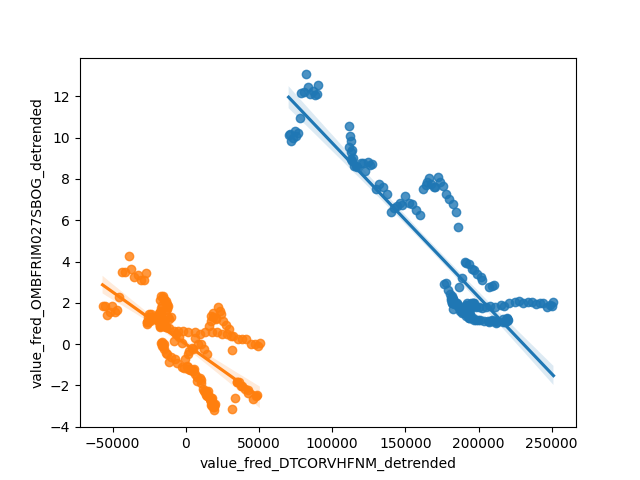
\includegraphics[scale = 0.9]{plots/plot_2026-10-28_detrended.png}
\caption{Detrended Regression Plot for 2026-10-28}
\end{figure}
\newpage
